\subsection{Simulation Methodology}
In order to reliably simulate multirotor parameters \textit{xcopterCalc}, a free tool provided by \textit{eCalc}, is utilized. This tool is widely used throughout the multirotor design community, with \textit{eCalc} being partnered with several prominent multirotor manufacturers (such as LeoMotion, DualSky, and more).

Through use of \textit{xcopterCalc}, differing model parameters (such as battery size, payload weight, and propeller selection) can be tweaked in order to obtain a reasonable estimate for the multirotor's actual flight performance. 

It is important to stress that the figures extracted from \textit{xcopterCalc} are only estimates. While the tool often makes conservative estimates (for example, a 3S 5000 mAh LiPo was measured to weigh 360 g while modeled to weigh 420 g in \textit{xcopterCalc}), the tool also neglects several real-world non-idealities. Such ignored non-idealities include high-frequency disturbances to control systems, and the electric power consumption of the flight control unit and its sensors. 

There also exists limitations regarding to the selection of motor and propeller models. The simulation calculates the driver performance of the motors (i.e. their power consumption and mechanical power output) through use of a database containing performance characteristics submitted by parts manufacturers. The motors and propellers ultimately purchased for the final implementation are not listed within this database, thus similar (near-identical) models are substituted for use within the simulation. Alternative motors within this database are discussed in Section \ref{prop_explore} to examine potential performance upgrades potentially available to the client in the future.

\subsection{Design Verification}
To verify the performance of the final part selection (as detailed in the \textit{Design Document}), two simulations were performed with differing model weights -- 1200g and 600g. The model weight denotes the weight of the system excluding the powertrain. In other words, the model weight denotes the combined weight of the drone frame, accessories, and computation platform (including the computation platform battery). Fixed design and environmental parameters, used across both tests, are listed in Table \ref{env_param}.

\begin{table}[H]
\label{env_param}
\centering
\begin{tabular}{|l|l|}
\hline
Number of Rotors    & 4        \\ \hline
Frame Size          & 560 mm   \\ \hline
Controller Amperage & 30 A     \\ \hline
Field Elevation     & 100 m    \\ \hline
Air Temperature     & 25$^{\circ}$ C     \\ \hline
Pressure            & 1013 hPa \\ \hline
\end{tabular}
\caption{Fixed Design and Environmental Parameters}
\end{table}

A screenshot of the simulation, outlining all expected parameters, is included in each section. A summary of the results is seen in Table \ref{summary}.

\begin{table}[]
\centering
\begin{tabular}{|l|l|l|}
\hline
\textbf{Model Weight (g)}              & \textbf{1200}       & \textbf{600}        \\ \hline
Battery Size                  & 3S 5000mAh & 3S 5000mAh \\ \hline
Hover Flight Time (min)       & 9.9        & 16         \\ \hline
Thrust:Weight Ratio           & 1.7        & 2.3        \\ \hline
Thrust (g/W)                  & 7.21       & 8.43       \\ \hline
Maximum Power Consumption (W) & 171.2      & 171.2      \\ \hline
\end{tabular}
\caption{Simulated Performance of Final Part Selection}
\label{summary}
\end{table}

\subsubsection{1200 g Model Weight Simulation}

\begin{figure}[H]
\centering
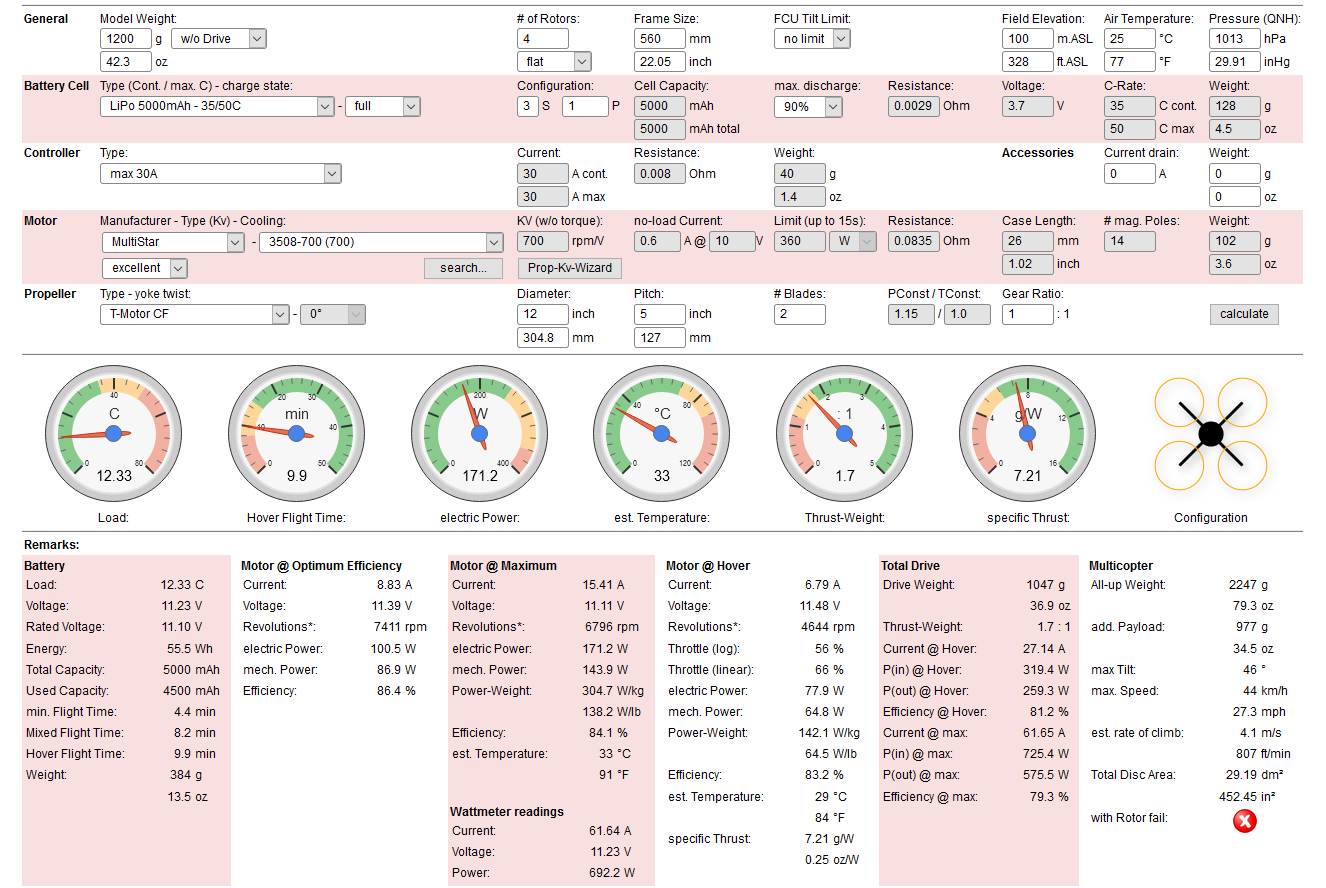
\includegraphics[width=16.5cm]{img/1200g_sim.png}
\caption{\textit{xcopterCalc} Output For 1200 g Model Weight}
\end{figure} 

\begin{figure}[H]
\centering
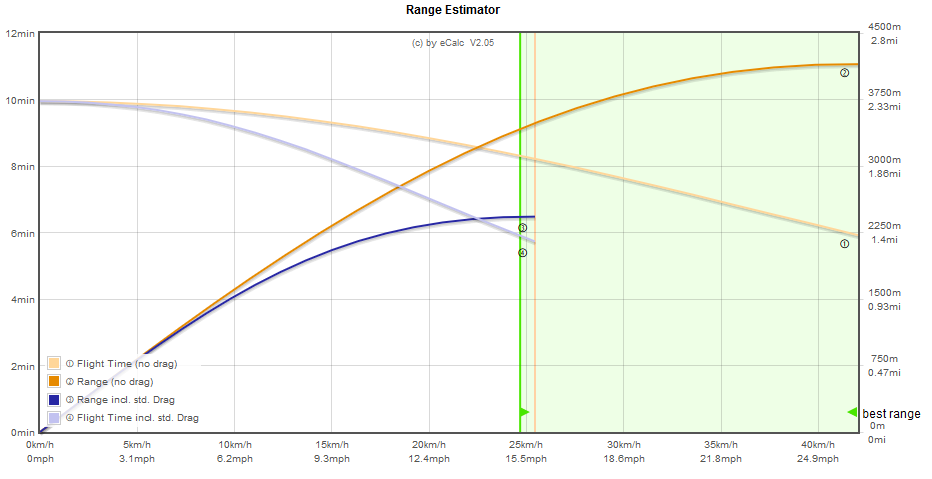
\includegraphics[width=16.5cm]{img/1200g_range.png}
\caption{Expected Range For 1200 g Model Weight}
\end{figure} 

\begin{figure}[H]
\centering
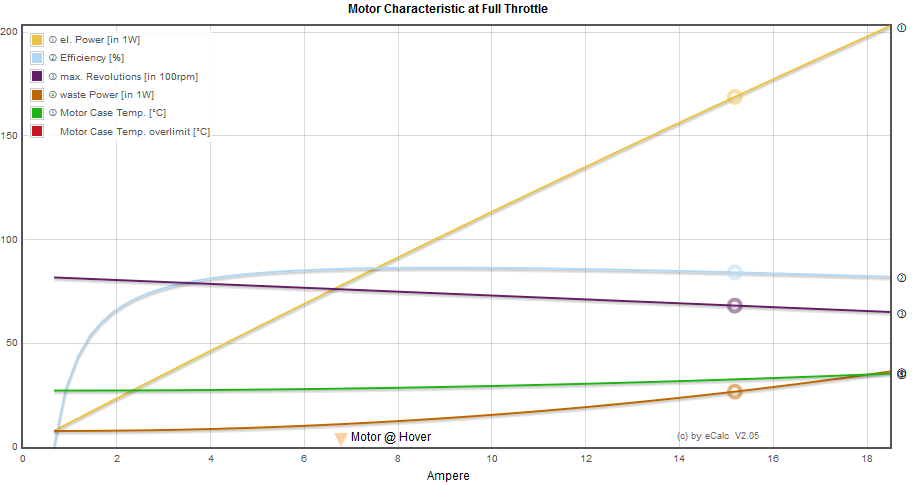
\includegraphics[width=16.5cm]{img/1200g_motor.png}
\caption{Motor Characteristics For 1200 g Model Weight}
\end{figure} 

\subsubsection{600 g Model Weight Simulation}

\begin{figure}[H]
\centering
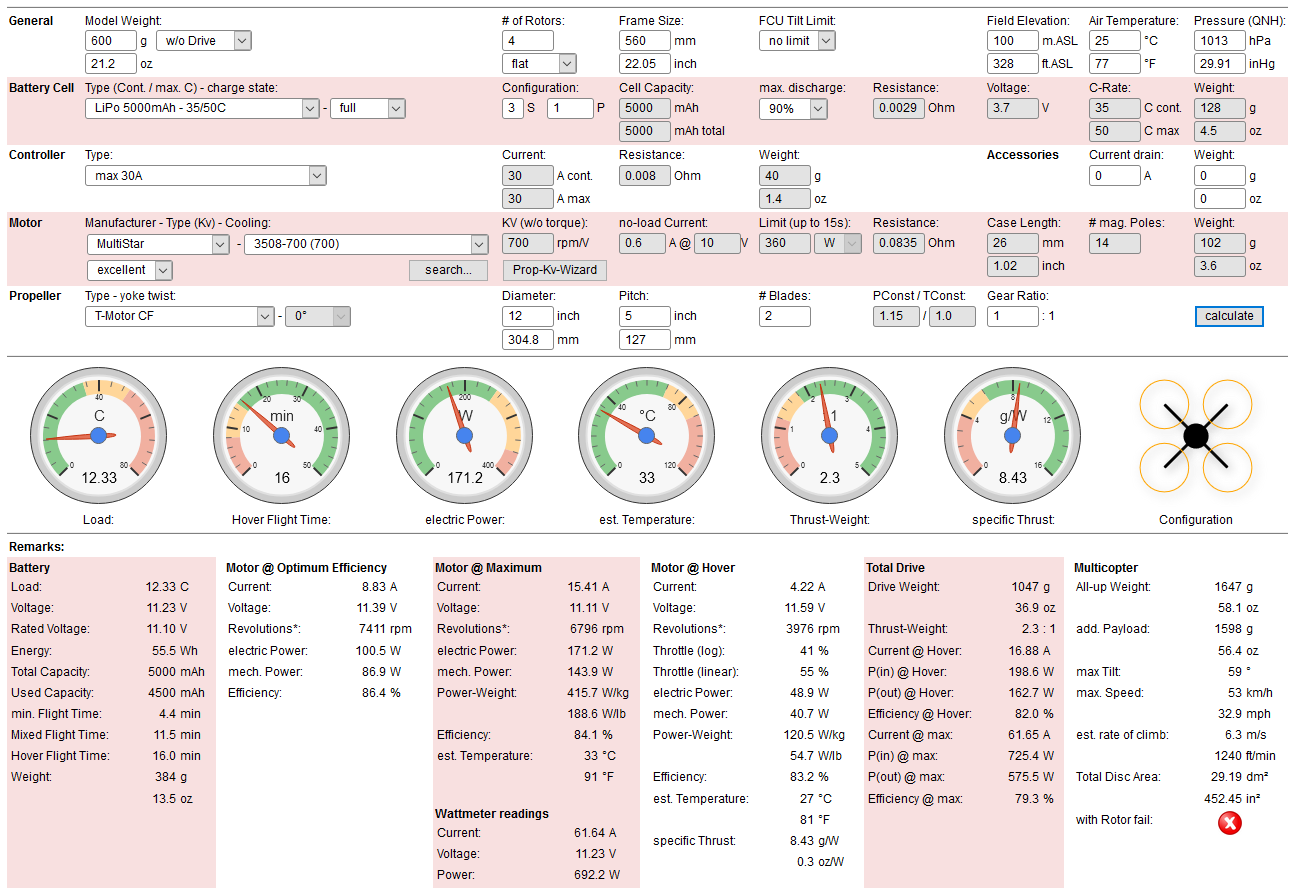
\includegraphics[width=16.5cm]{img/600g_sim.png}
\caption{\textit{xcopterCalc} Output For 600 g Model Weight}
\end{figure} 

\begin{figure}[H]
\centering
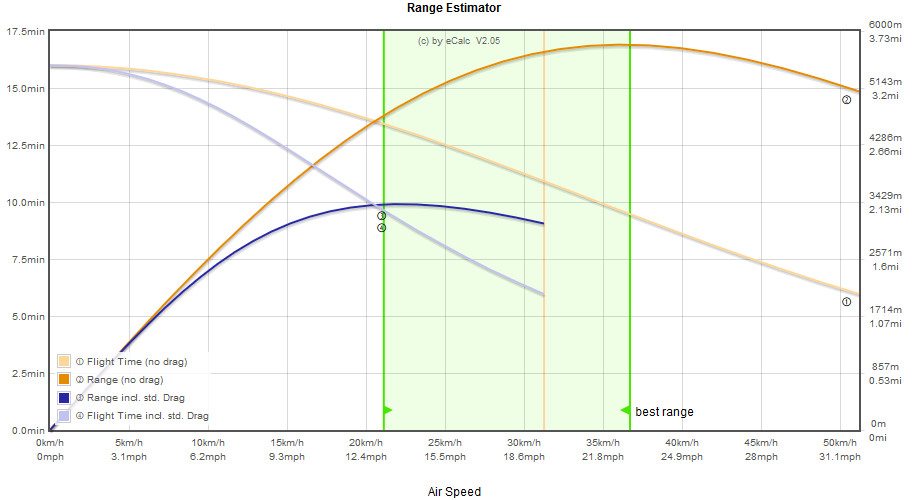
\includegraphics[width=16.5cm]{img/600g_range.png}
\caption{Expected Range For 600 g Model Weight}
\end{figure} 

\begin{figure}[H]
\centering
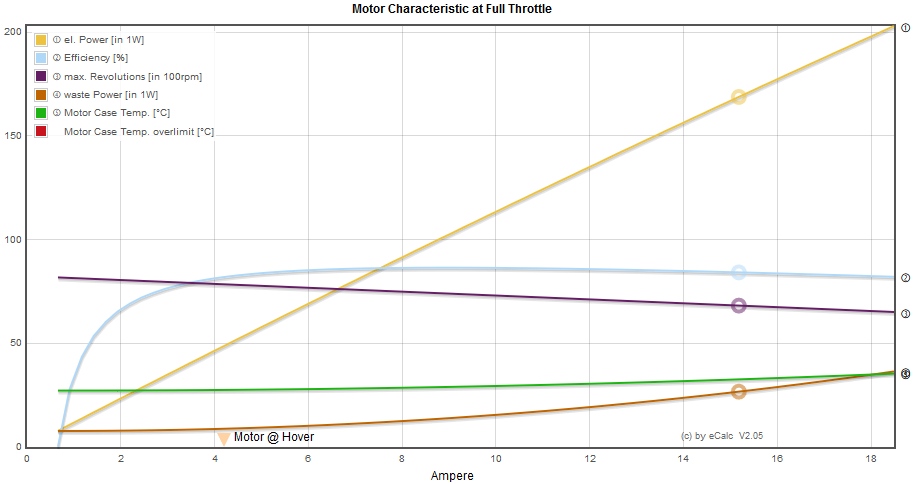
\includegraphics[width=16.5cm]{img/600g_motor.png}
\caption{Motor Characteristics For 600 g Model Weight}
\end{figure} 
\clearpage

\subsection{Payload Weight Variations}
As the client may wish to extend the functionality of the multirotor by adding or replacing components of the computing platform, simulations have been performed to provide insight as to the impact of payload weight on flight performance. In particular, the following simulations measure maximum hover time across differing model weights, battery configurations (ex. 3S/4S), and battery capacities (ex. 3000 to 10000 mAh). All other (non-weight-related) parameters are kept constant across tests.

\begin{figure}[H]
\centering
\begin{subfigure}{.5\textwidth}
\begin{tikzpicture}
\pgfplotsset{compat=1.3}
\centering
\begin{axis}[
  xlabel=Total Model Weight (grams),
  ylabel=Hover Time (minutes),
  ylabel shift = -5 pt]
\addplot table [y=flightduration, x=weight]{plots/3S-5000.txt};
\addlegendentry{5000 mAh}
\addplot table [y=flightduration, x=weight]{plots/3S-6000.txt};
\addlegendentry{6000 mAh}
\addplot table [y=flightduration, x=weight]{plots/3S-10000.txt};
\addlegendentry{10000 mAh}
\end{axis}
\end{tikzpicture}
\caption{Simulated Hover Times for 3S Batteries}
\end{subfigure}%
\begin{subfigure}{.5\textwidth}
\centering
\begin{tikzpicture}
\pgfplotsset{compat=1.3}
\begin{axis}[
  xlabel=Total Model Weight (grams),
  ylabel=Hover Time (minutes),
  ylabel shift = -5 pt]
\addplot table [y=flightduration, x=weight]{plots/4S-5000.txt};
\addlegendentry{5000 mAh}
\addplot table [y=flightduration, x=weight]{plots/4S-6000.txt};
\addlegendentry{6000 mAh}
\addplot table [y=flightduration, x=weight]{plots/4S-10000.txt};
\addlegendentry{10000 mAh}
\end{axis}
\end{tikzpicture}
\caption{Simulated Hover Times for 4S Batteries}
\end{subfigure}
\end{figure}

\subsection{Propulsion Performance Exploration}
\label{prop_explore}

In order to increase the effective range and flight duration of the multirotor, the client may wish to install higher-capacity batteries (in potentially alternate configurations). The following simulations sweep potential battery capacities and outline their impact on hover time, mixed flight time, and payload capacity.

\begin{figure}[H]
\centering
\begin{subfigure}{.5\textwidth}
\begin{tikzpicture}[scale=0.95]
\pgfplotsset{compat=1.3}
\centering
\begin{axis}[
  xlabel=Battery Capacity (mAh),
  ylabel=Flight Duration (minutes),
  ylabel shift = -5 pt,
  legend pos=south east]
\addplot table [y=hover, x=capacity]{plots/3S-time.txt};
\addlegendentry{Hover Flight}
\addplot table [y=mixed, x=capacity]{plots/3S-time.txt};
\addlegendentry{Mixed Flight}
\end{axis}
\end{tikzpicture}
\caption{3S Batteries}
\end{subfigure}%
\begin{subfigure}{.5\textwidth}
\centering
\begin{tikzpicture}[scale=0.95]
\pgfplotsset{compat=1.3}
\centering
\begin{axis}[
  xlabel=Battery Capacity (mAh),
  ylabel=Flight Duration (minutes),
  ylabel shift = -5 pt,
  legend pos=south east]
\addplot table [y=hover, x=capacity]{plots/4S-time.txt};
\addlegendentry{Hover Flight}
\addplot table [y=mixed, x=capacity]{plots/4S-time.txt};
\addlegendentry{Mixed Flight}
\end{axis}
\end{tikzpicture}
\caption{4S Batteries}
\end{subfigure}
\caption{Simulated Flight Times for Varying Battery Capacities}
\label{flighttime}
\end{figure}

\begin{figure}[H]
\centering
\begin{subfigure}{.5\textwidth}
\begin{tikzpicture}[scale=0.95]
\pgfplotsset{compat=1.3}
\centering
\begin{axis}[
  xlabel=Battery Capacity (mAh),
  ylabel=Weight (grams),
  legend style={at={(0.5,-0.1)},anchor=north},
  ylabel shift = -5 pt]
\addplot table [y=multirotor, x=capacity]{plots/3S-weight.txt};
\addlegendentry{Multirotor Weight}
\addplot table [y=payload, x=capacity]{plots/3S-weight.txt};
\addlegendentry{Payload Capacity}
\addplot table [y=total, x=capacity]{plots/3S-weight.txt};
\addlegendentry{Maximum Takeoff Weight}
\end{axis}
\end{tikzpicture}
\caption{3S Batteries}
\end{subfigure}%
\begin{subfigure}{.5\textwidth}
\centering
\begin{tikzpicture}[scale=0.95]
\pgfplotsset{compat=1.3}
\centering
\begin{axis}[
  xlabel=Battery Capacity (mAh),
  ylabel=Weight (grams),
  legend style={at={(0.5,-0.1)},anchor=north},
  ylabel shift = -5 pt]
\addplot table [y=multirotor, x=capacity]{plots/4S-weight.txt};
\addlegendentry{Multirotor Weight}
\addplot table [y=payload, x=capacity]{plots/4S-weight.txt};
\addlegendentry{Payload Capacity}
\addplot table [y=total, x=capacity]{plots/4S-weight.txt};
\addlegendentry{Maximum Takeoff Weight}
\end{axis}
\end{tikzpicture}
\caption{4S Batteries}
\end{subfigure}
\caption{Simulated Weights for Varying Battery Capacities}
\label{flightweight}
\end{figure}


As seen in Figure \ref{flighttime}, as battery capacity increases there is an asymptotic increase in both hover and mixed flight time. This asymptotic behaviour stems from the increased weight demands of the higher capacity batteries -- a trend also seen in Figure \ref{flightweight} where higher capacity batteries take up a majority of the maximum take-off weight.
